\section{Introduction}
% Random notes:
% \begin{itemize}
% \item Use \defn{defn} blocks to define terms, such as 
% \defn{hardware transactional memory}.  However, \defn{defn} 
% blocks should always have an accompanying definition.  Their
% use is a good mnemonic for remembering that one should define
% important terms.
% \item In text, \textit{italics} or \emph{emphasis} blocks
% are used to draw attention to an otherwise well-defined term
% or phrase.  
% \end{itemize}




As Moore's law plateaus~\cite{Vardi14} the transition
to multicore microprocessors is in full swing. High-performing concurrent
programs require the effective utilization of these multicore chips, but 
synchronization overhead and complexity has been a
major roadblock to building fast concurrent programs.
Transactional memory~\cite{HerlihyMo93} was originally
proposed as a programming abstraction that could achieve
high performance while maintaining the simplicity of 
coarse-grained locks~\cite{YooHuLa13}.
Recently, Intel~\cite{Reinders12,IntelISAX12} and
IBM~\cite{CainMiFr13,Merritt11,IBMPower8Overview14} have both
introduced mainstream multicores supporting restricted \defn{hardware
transactional memory} (HTM) and a new ingredient in the solution 
to the synchronization problem is on the horizon. The Intel and IBM
systems are both \emph{restricted} in that they are 
a \emph{best effort} hardware transactional memory
system~\cite{Roman12,IntelISAX12,CainMiFr13,IBMPower8Optimization14}.
This means that there is no guarantee that an attempted 
transaction will complete successfully, even in the absence 
of memory contention from other cores, due to hardware restrictions
arising from the imperfect implementation.  
Hardware transactions are faster than traditional
coarse-grained locks and software
transactions~\cite{YooHuLa13}~\cite{CascavalBlMi08}, 
yet they have similar
performance to well-engineered software using fine-grained 
locks and atomic instructions (e.g.
\proc{compare-and-swap}~\cite{Herlihy91})~\cite{YooHuLa13}. 
However, \emph{restricted} HTM introduces a wrinkle into 
this otherwise panacean technology: sometimes transactions
will fail even when executed serially due to limitations
of the underlying hardware implementation.  The conditions
under which such a failure may occur dramatically impacts
whether the complexity of designing a software 
system using restricted HTM
is justified by the expected performance.  Characterizing
these conditions is the goal of this paper. 

\begin{figure}[h]%[ht!]
\centering
\begin{minipage}[b]{.45\linewidth}
\centering
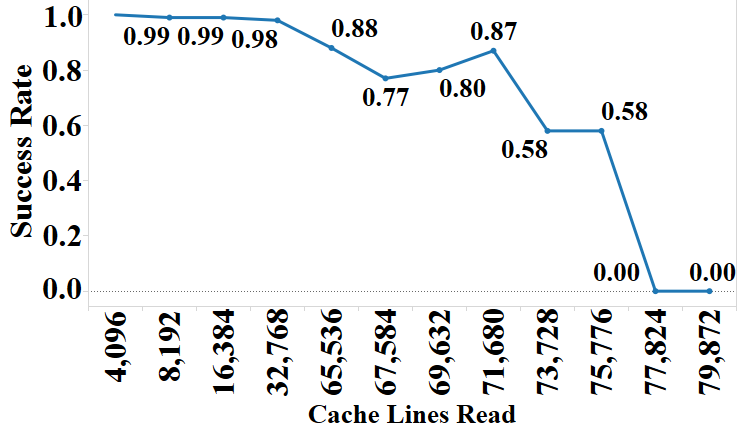
\includegraphics[width=\linewidth]{images/wttm_capacity_read_intel}
\caption{Lines Read vs Success Rate.}
\label{fig:wttm_capacity_read_intel}
\end{minipage}%
\quad
\begin{minipage}[b]{.45\linewidth}
\centering
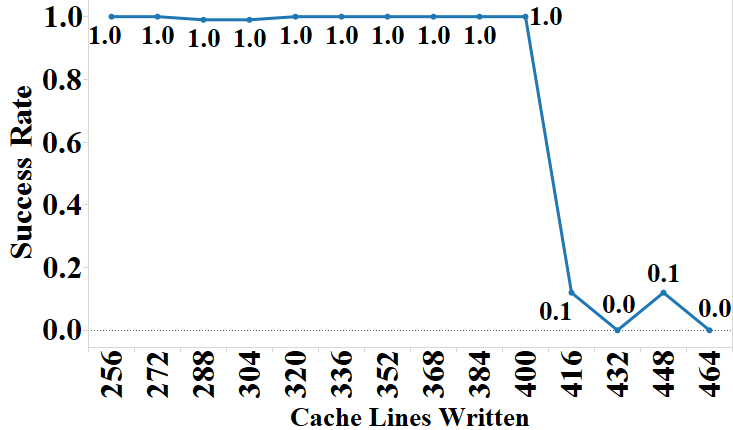
\includegraphics[width=\linewidth]{images/wttm_capacity_write_intel}
\caption{Lines Written vs Success Rate.}
\label{fig:wttm_capacity_write_intel}
\end{minipage}
\end{figure}

Transactions require the logical 
maintenance of \defn{read sets}, the set
of memory locations that are read within a 
transaction, and \defn{write sets}, the set
of memory locations that are written within 
a transaction~\cite{HerlihyMo93}. When transactions execute, 
local reads and writes to memory 
are tracked and recorded in
corresponding read and write sets. Upon 
completion of a transaction, the memory state is validated for 
consistency before the transaction
\defn{commits}, meaning that the modifications to 
memory are visible to other threads.


Transactions may \defn{abort} due to a conflict with
another concurrently executing transaction when an
inconsistent memory state is detected, 
such as when one or many memory locations
in one thread's write set intersects one or 
many memory locations in another
thread's read set or write set.  We call this a
\defn{conflict abort}.  In addition to \defn{conflict aborts},
hardware transactions specifically suffer 
from \textit{capacity aborts} when the underlying hardware
lacks sufficient resources to maintain the
read or write set.

\paragraph{Experimental Setup}
In this paper we summarize results of experiments 
that determine how the
read and write sets are maintained in hardware for recent 
Intel x86 and IBM PowerPC architectures. In particular,
the Intel machine contains a Haswell i7-4770 processor with 4
cores running at 3.4GHz, 8 hardware threads, 64B cache lines, an 8MB
16-way shared L3 cache, 256KB per-core 8-way L2 caches, 
and 32KB per-core 8-way L1 caches.
We also tested an IBM Power8 processor with 10 cores running at 3.4GHz,
80 hardware threads, 128B cache lines, an 80MB 8-way
shared L3 cache, and 64KB per-core 8-way L1 caches.
All experiments are written in C and compiled with GCC, 
optimization level
\texttt{-O0}.\footnote{We compiled with \texttt{-O0} because
we found that higher optimization levels sometimes 
caused spurious transaction
aborts, thus confounding our results.} Our experiments use the GCC
hardware transactional memory intrinsics interface.\footnote{The x86
intrinsics are \texttt{\_xbegin} and \texttt{\_xend}; 
the PowerPC intrinsics are
\texttt{\_\_builtin\_tbegin} and \texttt{\_\_builtin\_tend}.}

The focus of our experiments is to explore scenarios where these
capacity aborts are inevitable so that we know 
when hardware transactions are
not a feasible synchronization solution at all, 
even in the case of no contention. For example, 
\figreftwo{wttm_capacity_read_intel}{wttm_capacity_write_intel}
illustrate the maximum read and write capacity, respectively,
of a hardware transaction on an Intel processor.  In \secref{capacity}
we will explore other types of constraints imposed on
HTM operation by the Intel and IBM implementations.
This characterization should inform
software development attempting to use the newly available HTM support 
and hybrid hardware / software transactional memory
systems~\cite{DamronFeLe06,MatveevSh13}.
